% !TEX TS-program = pdflatex
% !TEX encoding = UTF-8 Unicode

% Matthew Urffer Master Thesis
% 
% Methods
%
\section{Simulation Methods}

%%%%%%%%%%%%%%%%%%%%%%%%%%%%%%%%%%%%%%%%%%%%%%%%%%%%%%%%%%%%%%%%%%%%%%%%%%%%%%%
%                                                                             %
%                             SIMULATION METHODS                              %
%                                                                             %
%%%%%%%%%%%%%%%%%%%%%%%%%%%%%%%%%%%%%%%%%%%%%%%%%%%%%%%%%%%%%%%%%%%%%%%%%%%%%%%
\subsection{MCNPX Simulations}
%%%%%%%%%%%%%%%%%%%%%%%%%%%%%%%%%%%%%%%%%%%%%%%%%%%%%%%%%%%%%%%%%%%%%%%%%%%%%%%
\begin{frame}{MCNPX Simulations}
	\centering
	\begin{figure}
		
\includegraphics[width=0.15\textwidth]{images/logo-mcnpx.eps}
	\end{figure}
\begin{itemize}
    \item MCNPX is a well validated transport code \cite{pelowitz_mcnpx_2010}
\end{itemize}
\tiny
    \newtheorem{thm10}{Dose Rate Calculation}
	\begin{thm10}<1->
		$$F2 = \frac{1}{A} \int_{A}{dA}\int_{E}{dE}\int_{4\pi}{d \Omega \Re(E) \Phi(\vec{r},E,\vec{\Omega})} $$
	where:
	\begin{itemize}
		\item $\Re(E)$ is the response function
		\item $\Phi(\vec{r},E,\vec{\Omega})$ is the photon flux
	\end{itemize}
	\end{thm10}
	\newtheorem{thm11}{Interaction Rate}
	\begin{thm11}<1->
		$$Q = C \int {\Phi(E) R_m(E) dE }$$
	where:
	\begin{itemize}
		\item $C$ is a scalar normalization (density)
		\item $R_m(E)$ is the response function
		\item $\Phi(E)$ is the neutron flux
	\end{itemize}
	\end{thm11}
\end{frame}

%%%%%%%%%%%%%%%%%%%%%%%%%%%%%%%%%%%%%%%%%%%%%%%%%%%%%%%%%%%%%%%%%%%%%%%%%%%%%%%
%                                                                             %
%                             SIMULATION VALIDATION                           %
%                                                                             %
%%%%%%%%%%%%%%%%%%%%%%%%%%%%%%%%%%%%%%%%%%%%%%%%%%%%%%%%%%%%%%%%%%%%%%%%%%%%%%%
\subsection{Simulation Validation}
%%%%%%%%%%%%%%%%%%%%%%%%%%%%%%%%%%%%%%%%%%%%%%%%%%%%%%%%%%%%%%%%%%%%%%%%%%%%%%%
\begin{frame}{Gamma Dose Rate Agreement}
\small
Compared simulated to measurements prefomed by RSO
	\begin{table}[h]
		\tiny
		\begin{tabular}{c c | c c}
        \multicolumn{2}{c}{Measured} & \multicolumn{2}{c}{Simulated} \\
        Distance (cm) & Dose Rate (mRem/hr) & Distance (cm) & Dose Rate (mRem/hr) \\
		\hline
		\hline
        10.2 & 10 & 10.2 & 10.3 \\
        13 & 5.5 & 12.7 & 5.38 \\
        28 & 2 & 28 & 1.80 \\
		\end{tabular}
	\end{table}
	\centering
	\begin{figure}
		\includegraphics[height=0.5\textheight]{images/DoseRate.eps}
		\caption{Dose Rate in Detector}
	\end{figure}
\end{frame}
%%%%%%%%%%%%%%%%%%%%%%%%%%%%%%%%%%%%%%%%%%%%%%%%%%%%%%%%%%%%%%%%%%%%%%%%%%%%%%%
\begin{frame}{Neutron Simulation Agreement}
	\begin{table}[h]
	\tiny
	\begin{tabular}{m{2cm} | >{\centering\arraybackslash}m{2cm} >{\centering\arraybackslash}m{2cm} >{\centering\arraybackslash}m{2cm}}
		 & Simulated Count Rate & Observed Count Rate & Relative Error \\
		 \hline
		 \hline
		 GS20 & 424.83 $\pm$ 3.8\% & 428 & -0.7 \% \\
		 PS Film, 25 $\mu$m & 56.23 $\pm$ 1.19\% & 51 & 9.5\% \\
		 PS Film, 50 $\mu$m & 108.10 $\pm$ 1.14\% & 96 & 12.6\% \\
	\end{tabular}
	\end{table}
	\tiny
	\begin{definition}[Relative Error]
		$$\sigma = \frac{\text{Obs} -\text{ Sim}}{\text{Obs}}$$
	where:
	\begin{itemize}
		\item $\text{Obs}$ is the observed count rate
		\item $\text{Sim}$ is the simulated count rate
	\end{itemize}
	\end{definition}
\end{frame}
